%% It is just an empty TeX file.
%% Write your code here.
% !TEX encoding = UTF-8 Unicode
\documentclass[a4paper, 12pt]{article}   	% use "amsart" instead of "article" for AMSLaTeX format
\usepackage[left=20mm, top=15mm, right=10mm, bottom=15mm]{geometry}    

            
\usepackage[parfill]{parskip}    		% Activate to begin paragraphs with an empty line rather than an indent
\usepackage{graphicx}				% Use pdf, png, jpg, or eps§ with pdflatex; use eps in DVI mode
\usepackage[14pt]{extsizes}
\usepackage{setspace,amsmath}
\usepackage{ dsfont }
\usepackage{graphicx}
\usepackage{amsmath,amssymb}
\usepackage[unicode]{hyperref}

\usepackage{xcolor}
\usepackage{color}
\usepackage{minted}
\usepackage{caption}

\usepackage{array}
\newcolumntype{P}[1]{>{\centering\arraybackslash}p{#1}}

\usepackage{cmap} % Улучшенный поиск русских слов в полученном pdf-файле
\usepackage[T2A]{fontenc} % Поддержка русских букв
\usepackage[utf8]{inputenc} % Кодировка utf8
\usepackage[english, russian]{babel} % Языки: русский, английский

								% TeX will automatically convert eps --> pdf in pdflatex		
\usepackage{amssymb}

\begin{document}
\begin{titlepage}

\thispagestyle{empty}

\begin{center}
Федеральное государственное бюджетное образовательное учреждение высшего профессионального образования Московский государственный технический университет имени Н.Э. Баумана
\end{center}


\vfill

\centerline{\large{Лабораторная работа}}

\centerline{\large{«Исследование экстремальных задач»}}

\centerline{\large{по курсу}}
\centerline{\large{«Методы оптимизации»}}


\vfill

Студент группы ИУ9-82 \hfill Белогуров А.А.

Преподаватель \hfill Каганов Ю.T.
\vfill

\centerline{Москва, 2018}
\clearpage
\end{titlepage}

\newpage
\setcounter{page}{2}

\tableofcontents

\newpage

\section{Цель работы}

\begin{enumerate}
    \item Знакомство с основными понятиями экстремальных задач.
    \item Исследование типов экстремумов для задач без ограничений.
    \item Исследование типов экстремумов для задач с ограничениями.
\end{enumerate}

\newpage

\section{Постановка задачи}

    \subsection{Задание 1}
    Построить график поверхности
    \begin{equation*}
        f(x_1, x_2) = a (x^2_1-1)^2 - b(x_2+5)^2, \quad a= 30, b = 2
    \end{equation*}
    и исследовать линии уровня для функций:
    \begin{equation*}
        f(x_1, x_2) = a (x^2_1-1)^2 - b(x_2+5)^2 = r^2, \quad a= 30, b = 2, r = 1,2,3,4.
    \end{equation*}

    \subsection{Задание 2}
    \begin{enumerate}
        \item Исследовать типы экстремумов для многоэкстремальных задач.
        \item Выявить экстремумы типа минимума и максимума.
        \item Определить локальные и глобальные экстремумы.
    \end{enumerate}
    
    Рассмотреть функцию Стенгера: 
    \begin{equation*}
        f(x_1, x_2) = (x_1^2 - 2x_2)^2 + (x_2^2 - 3x_1 + 4x_2)^2
    \end{equation*}
    в области поиска $x_i \in [-1, 4]$ при $a = -2$, $b = -3$, $c = 4$.

\subsection{Задание 3}
    Исследовать экстремальные задачи с заданными ограничениями. Найти точки условного экстремума для целевой функции:
    \begin{equation*}
        f(x_1, x_2) = x_1^2 + x_2^2, \quad X = \{x | x_2^2 - x_1 + 3 = 0 \}
    \end{equation*}

\newpage

\section{Исследование}

\subsection{Задание 1}
    Построить поверхность:
    \begin{equation*}
        f(x_1, x_2) = 30 (x^2_1-1)^2 - 2(x_2+5)^2
    \end{equation*}
    
    \begin{center}
        \begin{minipage}{0.47\linewidth}
            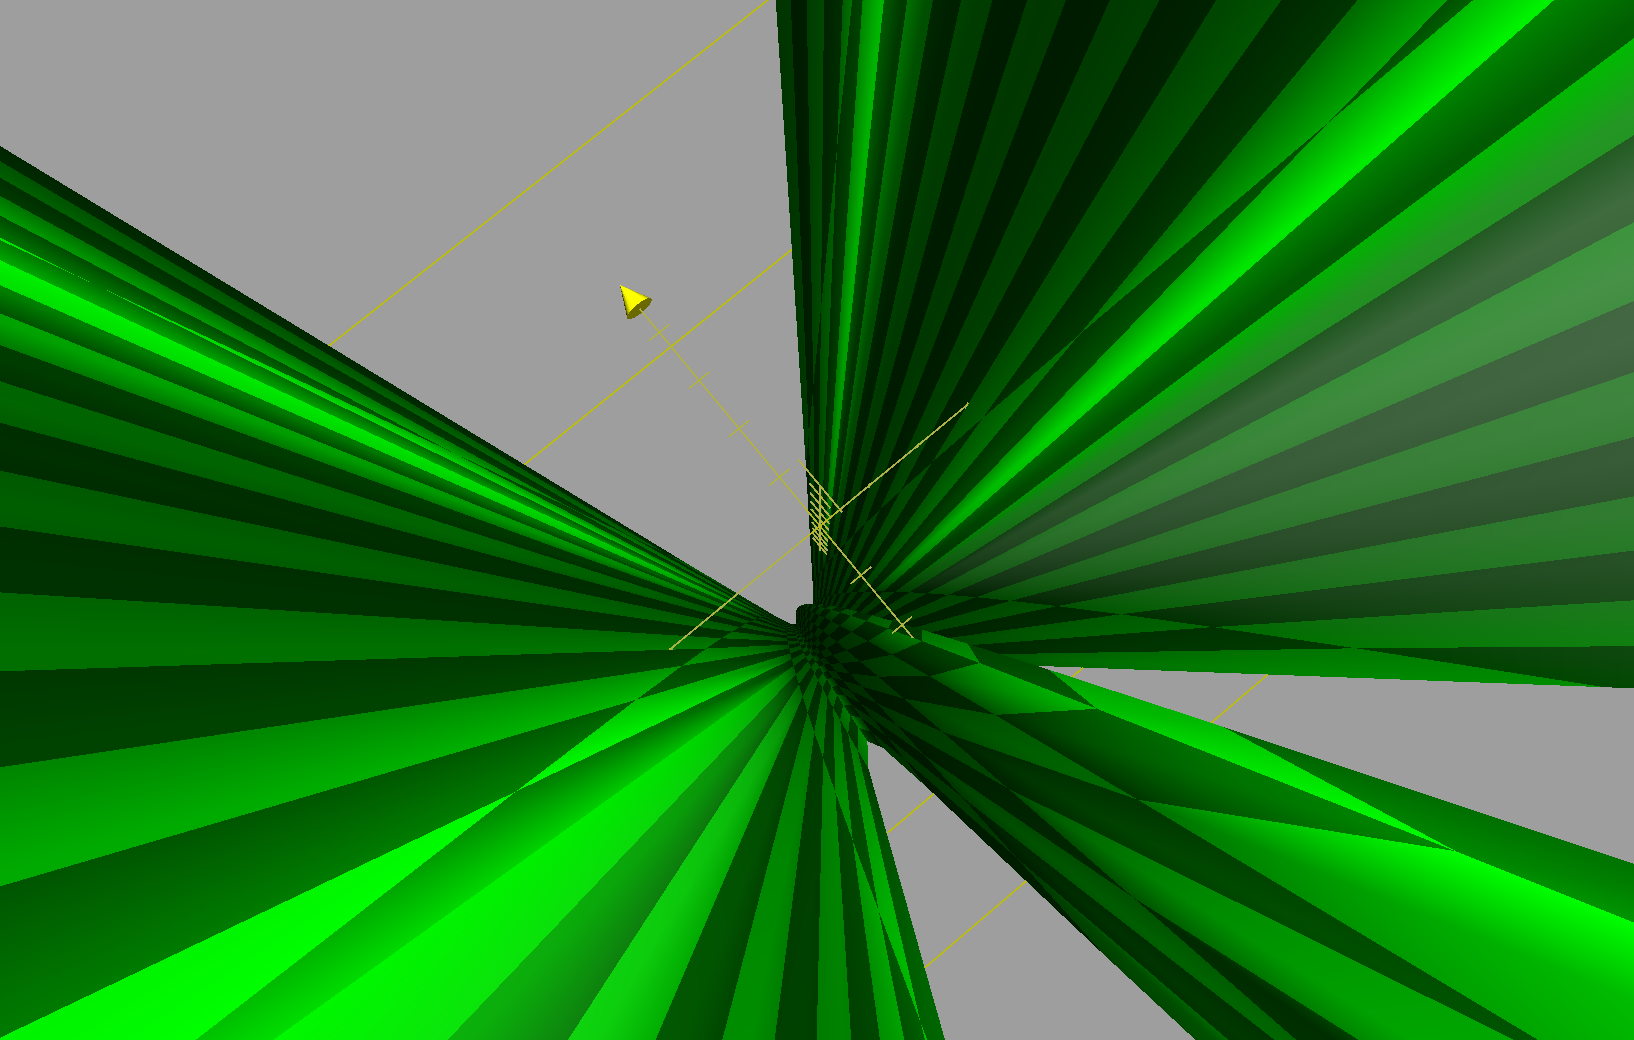
\includegraphics[width=\linewidth]{img/1_upper_view}
            \captionof{figure}{Вид сверху}
        \end{minipage}
        \begin{minipage}{0.47\linewidth}
            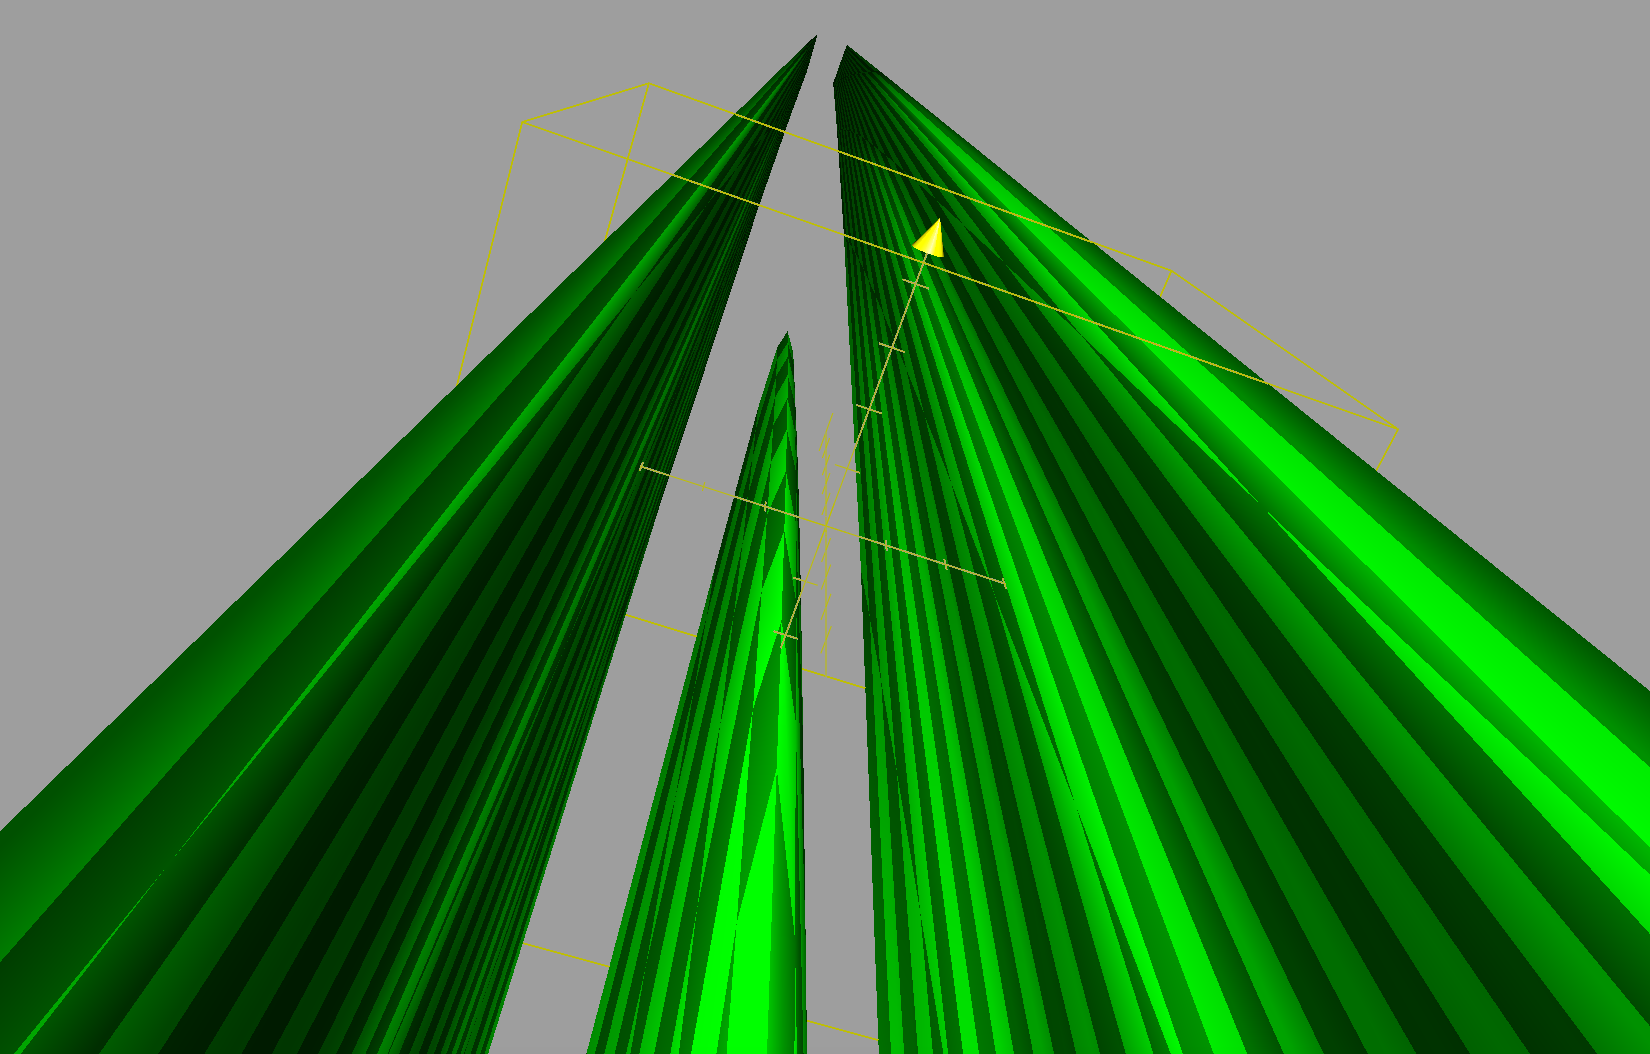
\includegraphics[width=\linewidth]{img/1_down_view}
            \captionof{figure}{Вид снизу}
        \end{minipage}
    \end{center}

    Построить линии уровня:
    \begin{equation*}
        f(x_1, x_2) = 30 (x^2_1-1)^2 - 2(x_2+5)^2 = r^2
    \end{equation*}
    
    \begin{center}
        \begin{minipage}{0.47\linewidth}
            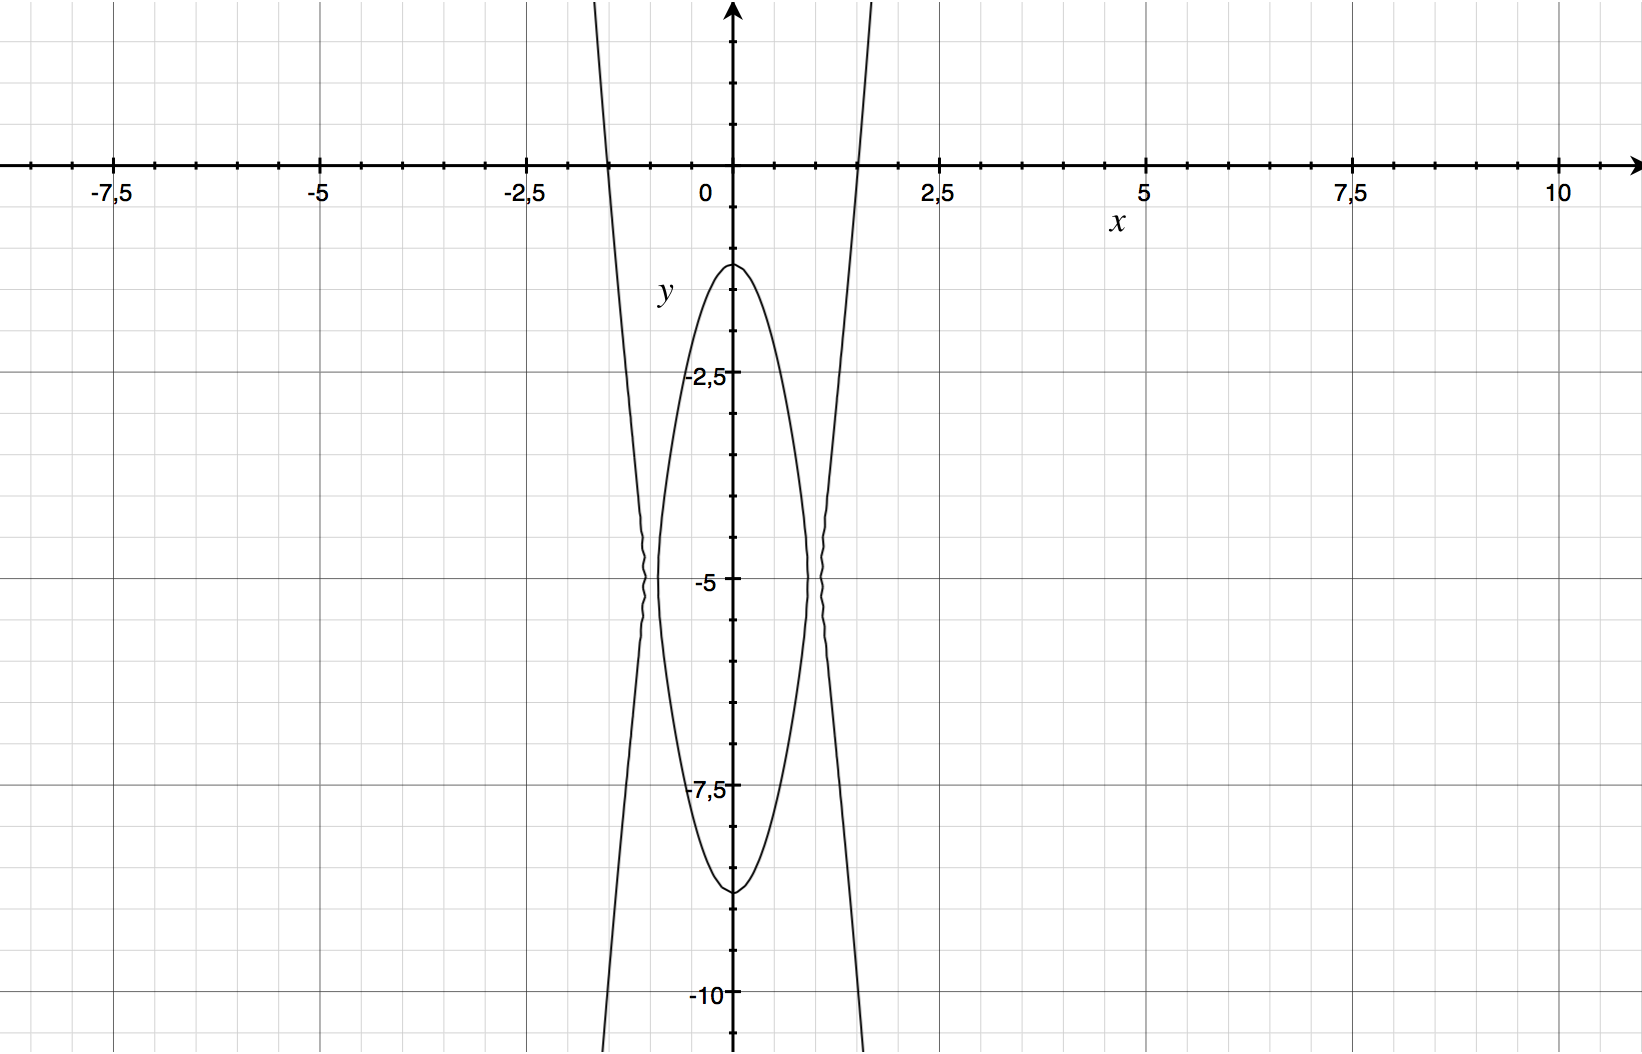
\includegraphics[width=\linewidth]{img/1_r1}
            \captionof{figure}{$\quad r = 1$}
        \end{minipage}
        \begin{minipage}{0.47\linewidth}
            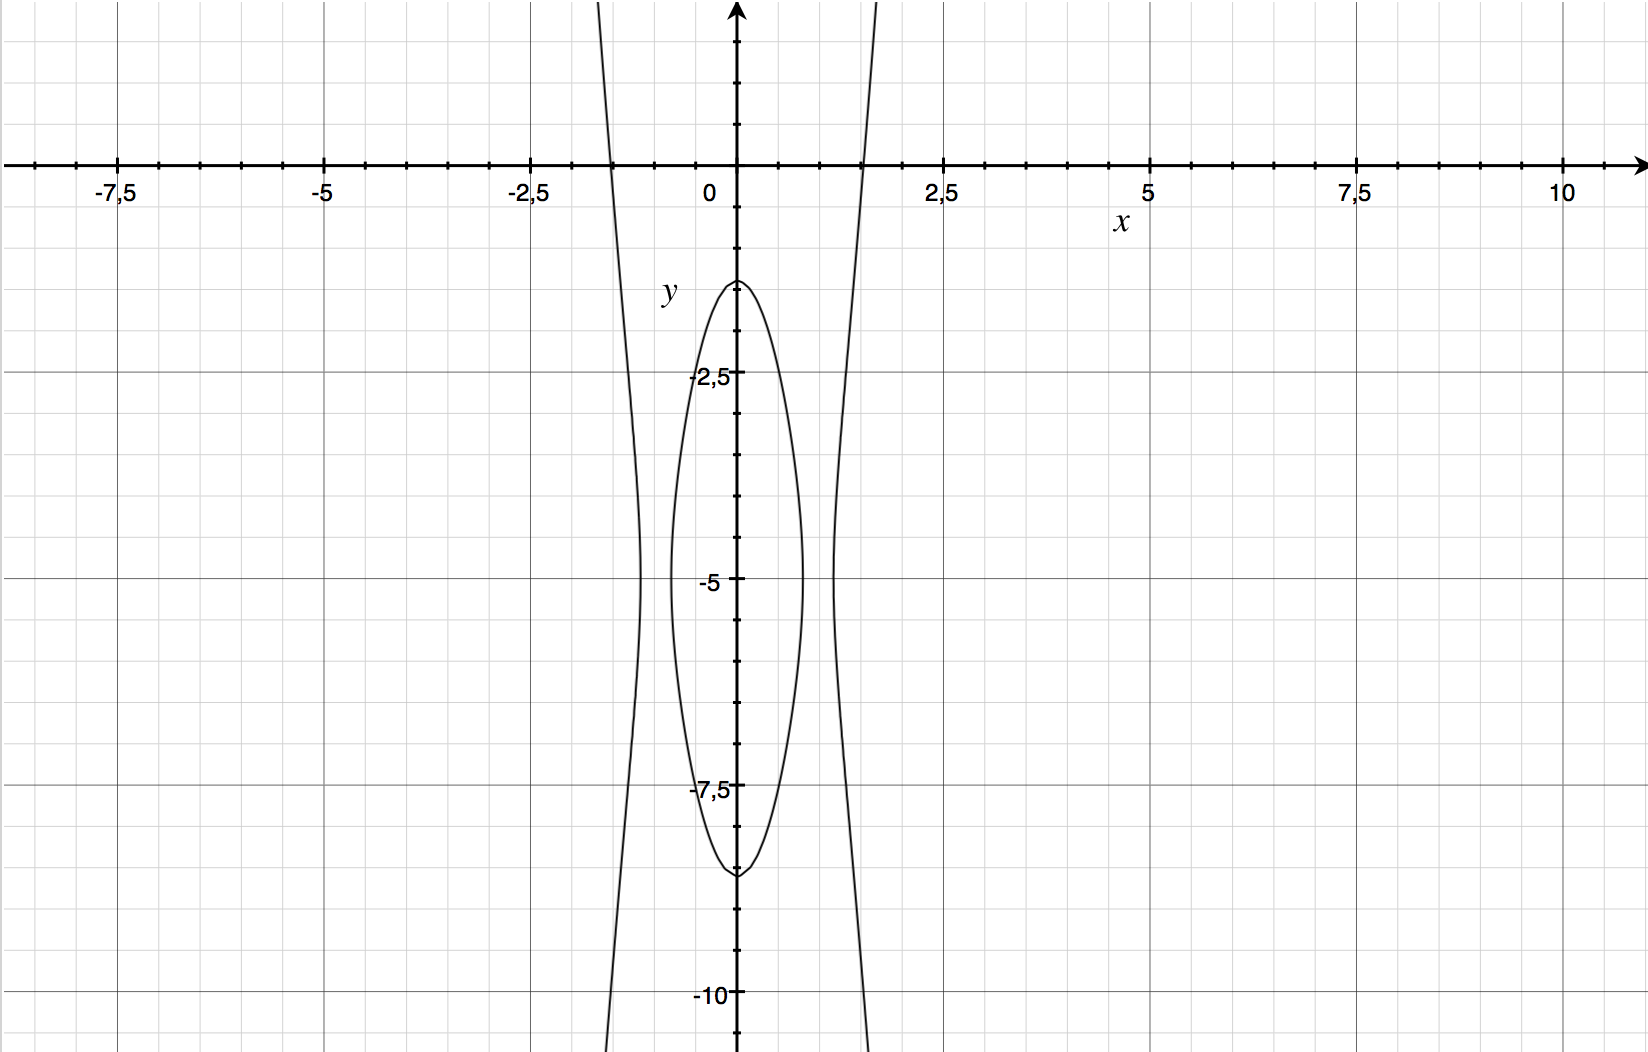
\includegraphics[width=\linewidth]{img/1_r2}
            \captionof{figure}{$\quad r=2$}
        \end{minipage}
        
        \begin{minipage}{0.47\linewidth}
            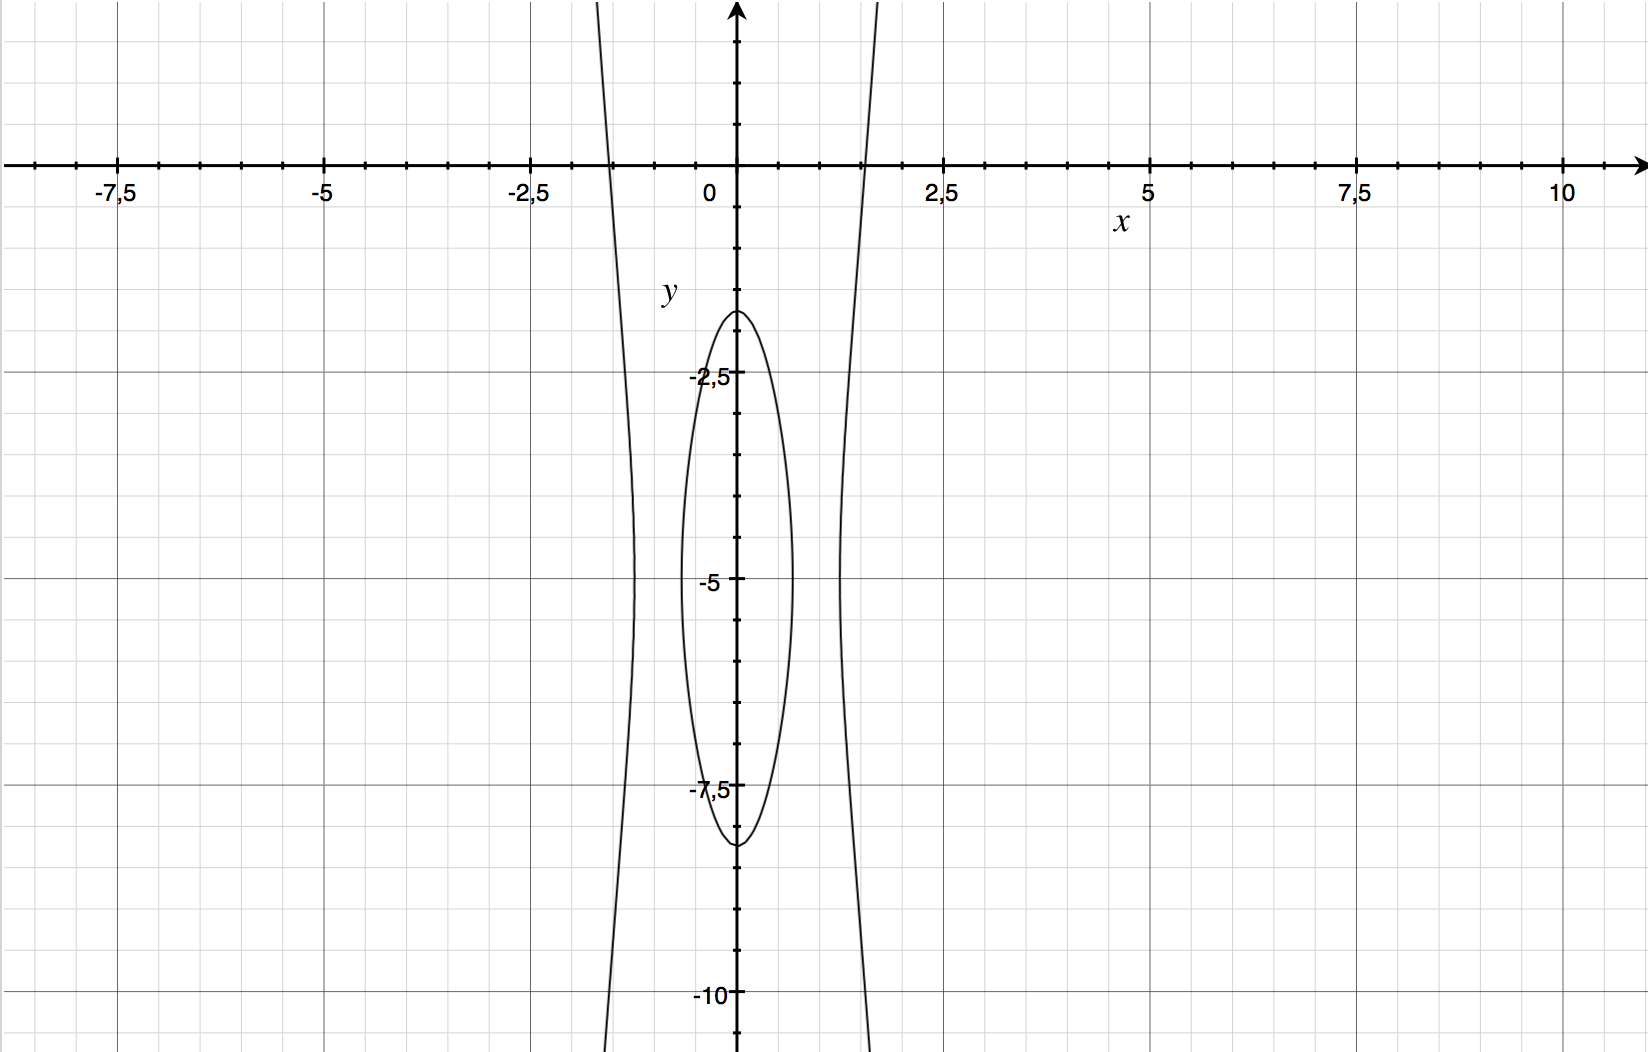
\includegraphics[width=\linewidth]{img/1_r3}
            \captionof{figure}{$\quad r = 3$}
        \end{minipage}
        \begin{minipage}{0.47\linewidth}
            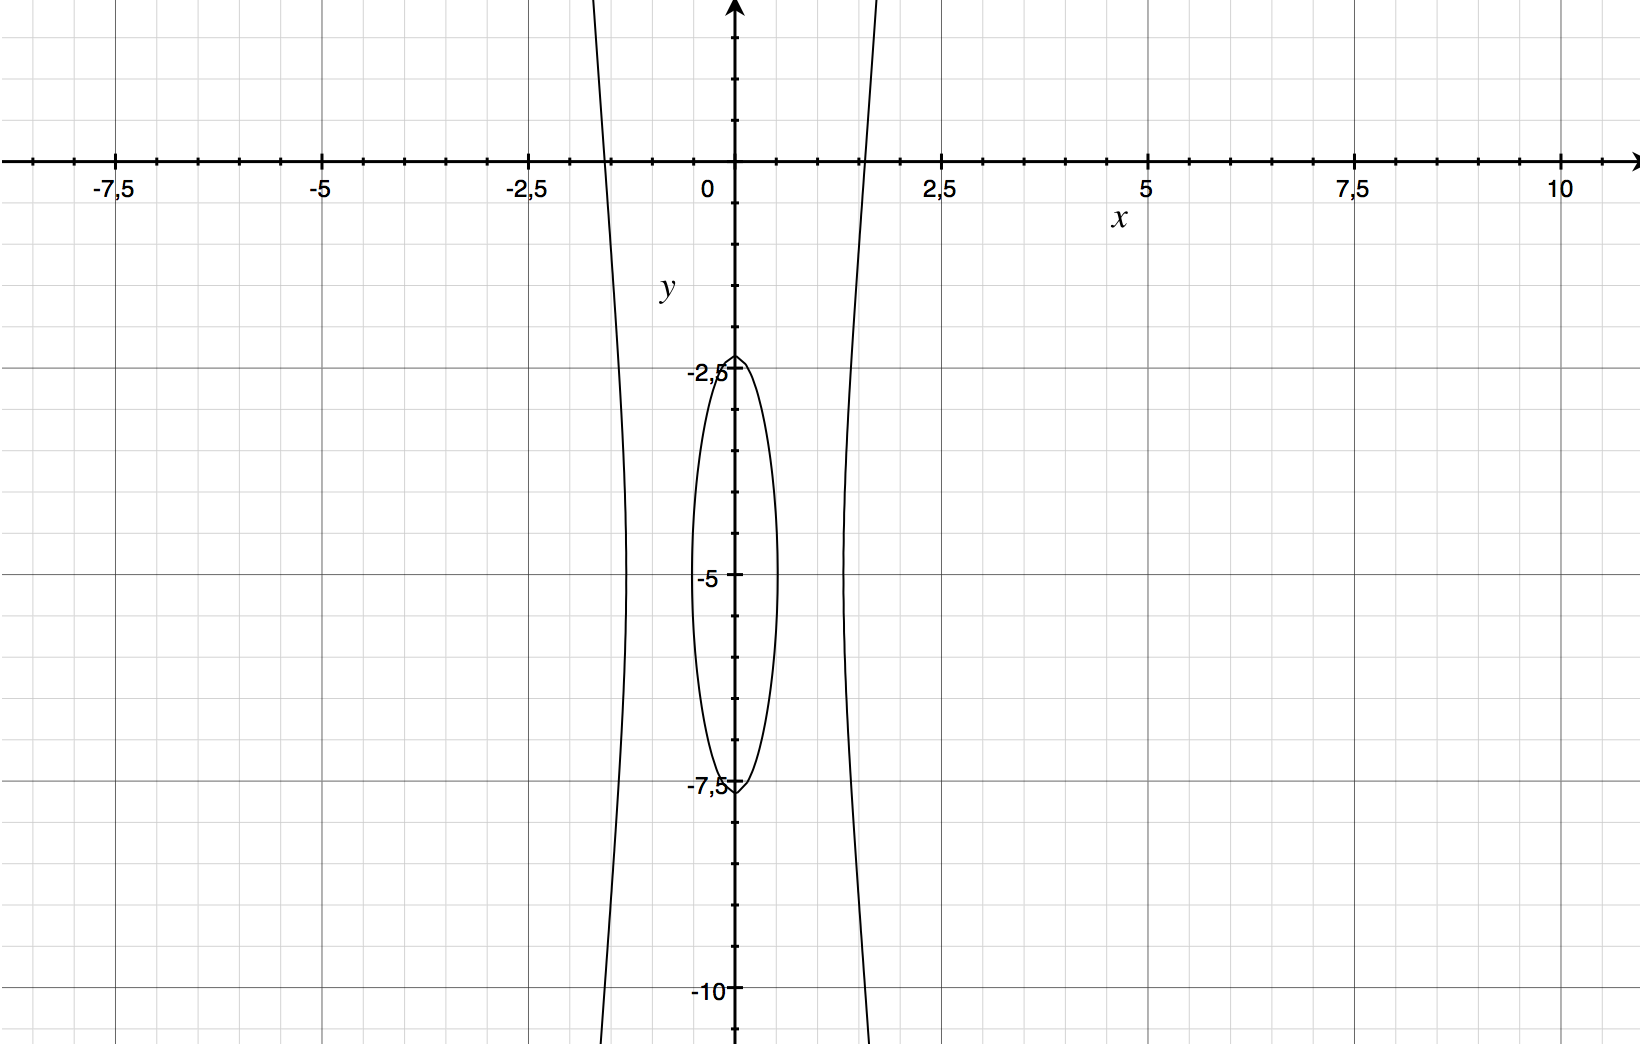
\includegraphics[width=\linewidth]{img/1_r4}
            \captionof{figure}{$\quad r=4$}
        \end{minipage}
    \end{center}
    
\subsection{Задание 2}

    Исследовать функицию
    
    \begin{equation*}
        f(x_1, x_2) = (x_1^2 - 2x_2)^2 + (x_2^2 - 3x_1 + 4x_2)^2 = 
    \end{equation*}
    \begin{equation*}
        = x_1^4-4x_1^2 x_2+9x_1^2-6x_1x_2^2 - 24x_1 x_2 + x_2^4 + 8 x_2^3 + 20 x_2^2
    \end{equation*}

    на глобальные и локальные экстремумы в области $x_i \in [-1, 4]$.
    
    Для нахождения этих точек был использован сервис WolframAlpha.com.
    
    \begin{enumerate}
        \item Глобальные экстремумы:
        \begin{itemize}
            \item $max(f(x_1, x_2)) = 1274$ в точке (-1, 4)
            \item $min(f(x_1, x_2)) = 0$ в точке - (0, 0)
            \item $min(f(x_1, x_2)) = 0$ в точке (1.25, 0.79)
         \end{itemize}
         \item Локальные экстремумы:
         \begin{itemize}
             \item $max(f(x_1, x_2)) = 9$ в точке (-1, -1)
             \item $min(f(x_1, x_2)) = 0$ в точке - (0, 0)
             \item $min(f(x_1, x_2)) = 0$ в точке (1.25, 0.79)
         \end{itemize}
    \end{enumerate}
    
    \begin{center}
        \begin{minipage}{0.5\linewidth}
            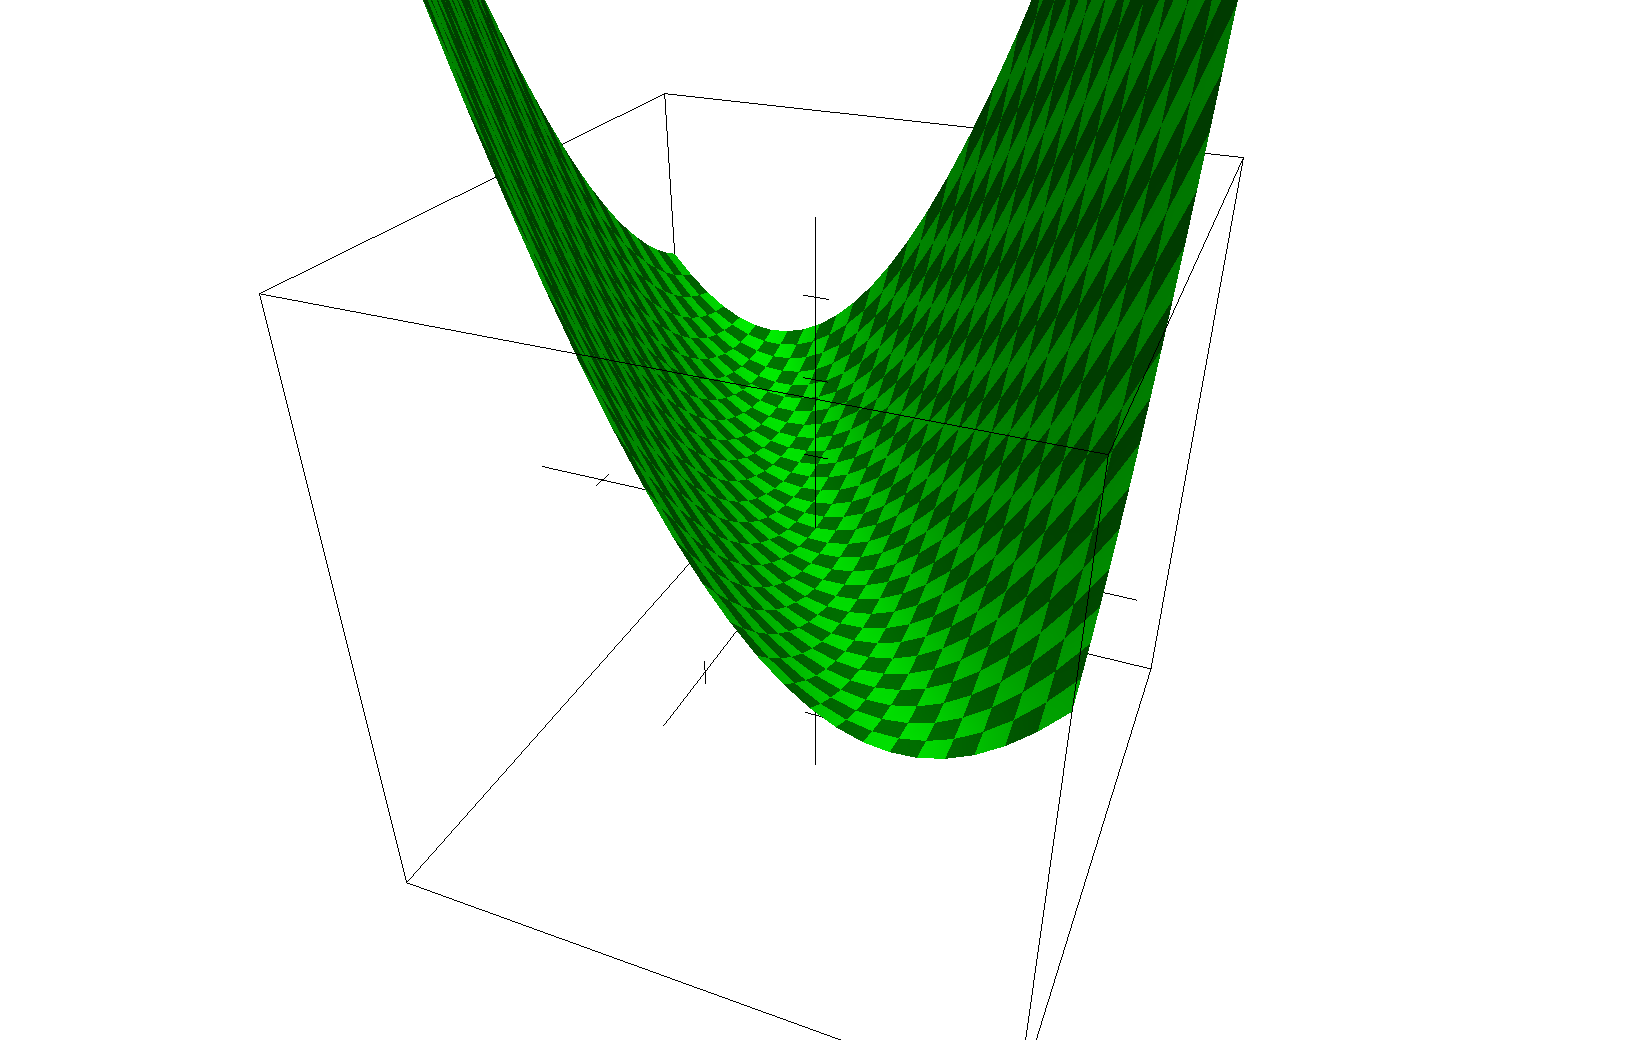
\includegraphics[width=\linewidth]{img/2}
            \captionof{figure}{График функции $f(x_1, x_2)$}
        \end{minipage}
    \end{center}
    
\subsection{Задание 3}
    
    Исследовать экстремальные задачи с заданными ограничениями. Найти точки условного экстремума для целевой функции:
    \begin{equation*}
        f(x_1, x_2) = x_1^2 + x_2^2, \quad X = \{x | x_2^2 - x_1 + 3 = 0 \}
    \end{equation*}
   
   \begin{enumerate}
        \item Экстремумы при ограничениях:
        \begin{itemize}
            \item $min(f(x_1, x_2)) = 9$ в точке - (3, 0)
        \end{itemize}
    \end{enumerate}
    
    \begin{center}
        \begin{minipage}{0.5\linewidth}
            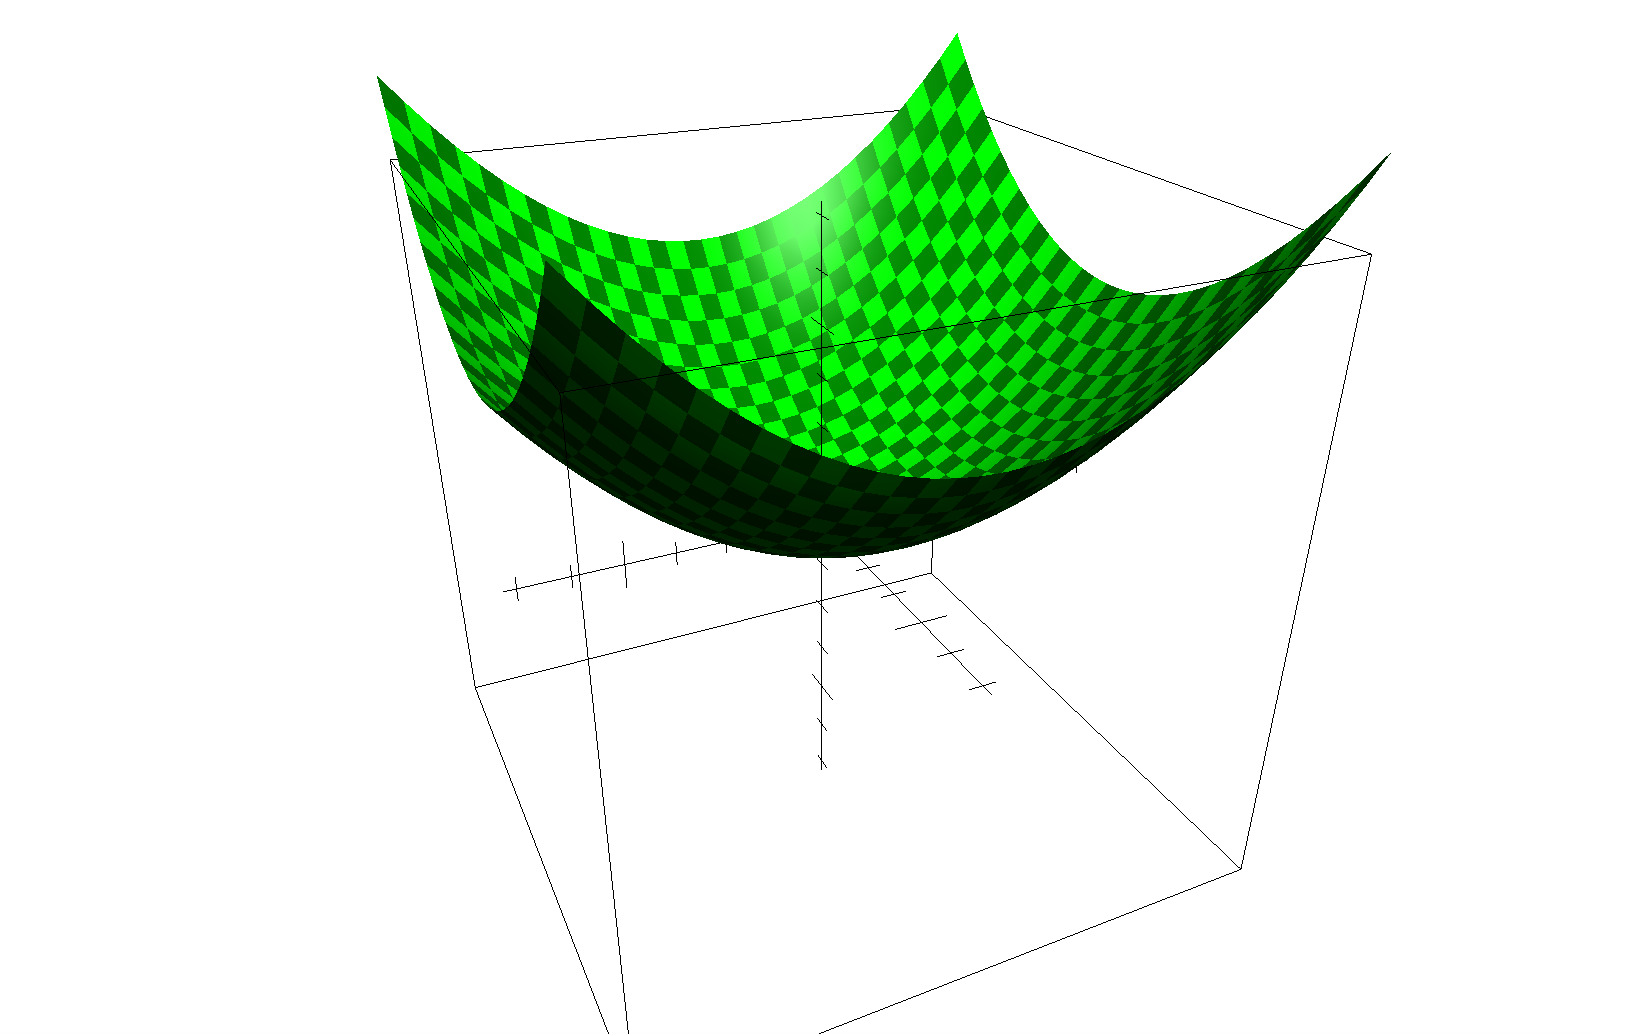
\includegraphics[width=\linewidth]{img/3}
            \captionof{figure}{График функции $f(x_1, x_2)$}
        \end{minipage}
    \end{center}
    
    

\end{document} 



